\documentclass[10pt]{beamer}

\usetheme{metropolis}
\usepackage{appendixnumberbeamer}
\usepackage{graphicx}
\usepackage{booktabs}
\usepackage[scale=2]{ccicons}
\usepackage{biblatex}
%\usepackage{pgfplots}
%\usepgfplotslibrary{dateplot}
\addbibresource{GeneticAlgorithms.bib}
\usepackage{xspace}
\usepackage[justification=centering]{caption}
\usepackage{algorithm}
\usepackage[noend]{algpseudocode}
\usepackage[version=3]{mhchem}
\newcommand{\themename}{\textbf{\textsc{metropolis}}\xspace}
\definecolor{darkgreen}{RGB}{30, 133, 12}


\title{Finding Many Stable Molecular Arrangements}
\subtitle{Conformational Searching with Genetic Algorithms}
\date{\today}
\author{Evan Curtin}
\institute{University of Illinois at Urbana-Champaign}

\begin{document}

\maketitle

\begin{frame}{Outline}
  \setbeamertemplate{section in toc}[sections numbered]
  \tableofcontents[hideallsubsections]
\end{frame}

\section{Background Information}

\begin{frame}[fragile]{The Problem}
	\begin{itemize}[<+->]
		\item[] {Computational methods require knowledge of molecular structure}
		\begin{itemize}
			\item[$\Rightarrow$] {We need to find the lowest energy structure}
		\end{itemize}
		\item[] {The potential energy surface (PES) is high dimensional and has many minima}
		\begin{itemize}
			\item[$\Rightarrow$] {We can't tell for sure if we've found the \alert{\textbf{global}} minimum}
		\end{itemize}
		\item[] {We may need information about one or more low-energy conformations}
		\begin{itemize}
			\item[$\Rightarrow$] {Ok, let's find them all!}
		\end{itemize}	
	\end{itemize}
\end{frame}

{%
\setbeamertemplate{frame footer}{Supady, A.; Blum, V.; Baldauf, C. J. Chem. Inf. Model. 2015, 55 (11), 2338–2348.}
\begin{frame}[fragile]{Possible Solutions}
	\begin{itemize}[<+->]
		\item[] {Many techniques are well established}
		\item[] {None are perfect}
	\end{itemize}
	\begin{figure}
		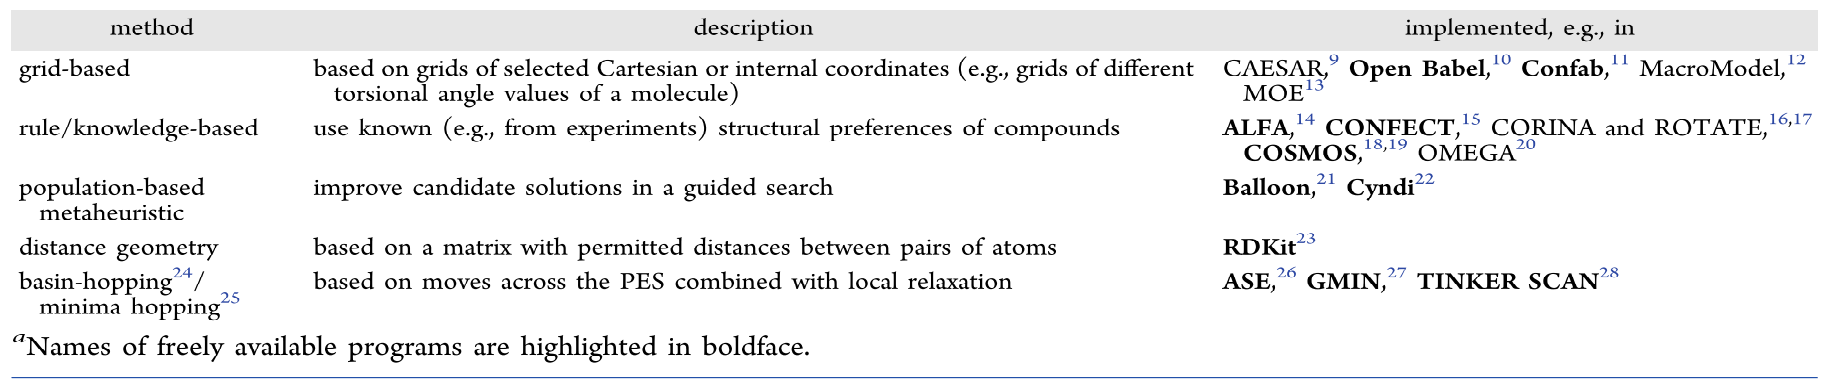
\includegraphics[width=\linewidth]{images/ImplementationTables.PNG}
	\end{figure}
\end{frame}
}

\begin{frame}{Desirables}
	\begin{itemize}[<+->]
		\item Accurate energies \& Structures, \emph{ab initio} or DFT
		\item {Minimize number of geometry optimizations}
		\item {Find the entire low energy population of conformations}
		\item {Minimal human input}
		\item {Parallel-Scalable}
	\end{itemize}	
\end{frame}

\section{The Genetic Algorithm}

{%
	\setbeamertemplate{frame footer}{Carwright, H. Reviews in Computational Chemistry 2007 (25), pp 349–389.}
\begin{frame}{Outline}
	\begin{columns}[c] % align columns
		\begin{column}{.48\textwidth}
			\begin{itemize}
				\item {Inspired by biological evolution}
				\item {Evolve a population over generations}
				\item {Survival of the fittest}
				\item {Requirements:}
				\begin{itemize}
					\item {Represent individuals as vector}
					\item {Fitness function}
				\end{itemize}
				\item{$v = \left(\begin{smallmatrix}
					x_1 & y_1 & z_1 & x_2 &  y_2 & z_2 &
					... & x_N & y_N & z_N
					\end{smallmatrix}\right)$}
				\item{$F = \frac{E_{max} - E}{E_{max} - E_{min}}$}
			\end{itemize}

		\end{column}
		\hfill
		\begin{column}{0.48\textwidth}
			\begin{figure}
			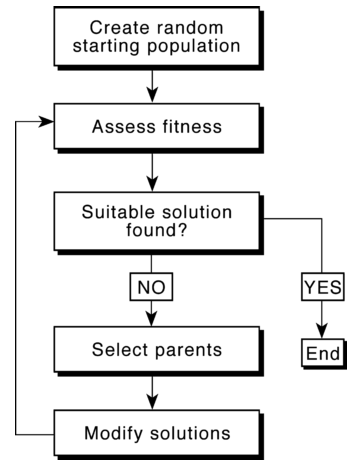
\includegraphics[width=0.8\linewidth]{images/GA_outline_Carwright.PNG}
			\end{figure}
		\end{column}	
	\end{columns}
\end{frame}
}

{%
\setbeamertemplate{frame footer}{1. Supady, A.; Blum, V.; Baldauf, C. J. Chem. Inf. Model. 2015, 55 (11), 2338–2348.
		
2. http://www.chemspider.com/Chemical-Structure.2298795.html}
\begin{frame}{From Structure to Vector}
	\begin{columns}[c] % align columns
		\begin{column}{.48\textwidth}
			\begin{itemize}
				\item<1-> {Several Ways to Define Structure
					\begin{itemize}
						\item[] {Cartesian}
						\item[] {Internal Coordinates (bond length, angle ...)}
						\item[] {SMILES, InChI}
					\end{itemize}
				}
				\item<2-> {InChI$^2$= 1S/C8H16/c1-5-7(3)8(4)6-2/h5-6H2,1-4H3/b8-7-}
				\item<only@3> {Equivalent in theory}
				\item<only@4> {Equivalent \alert{\textbf{in theory}}}
			\end{itemize}			
		\end{column}
		\hfill
		\begin{column}{0.48\textwidth}
			\begin{figure}
				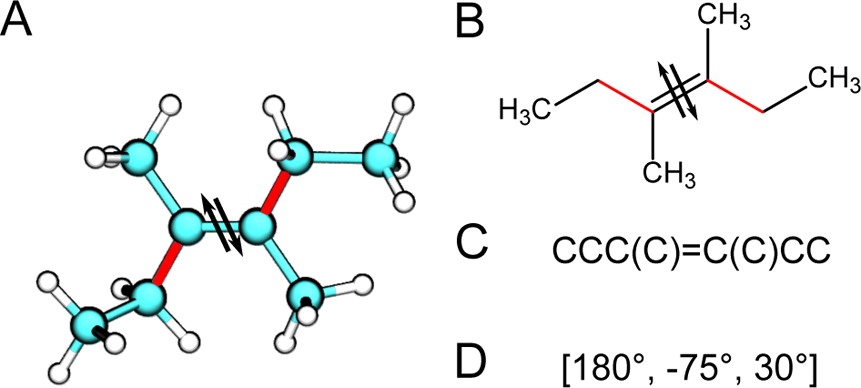
\includegraphics[width=0.95\linewidth]{images/Supady1.jpeg}
				\caption*{Representations of (3Z)-3,4-Dimethyl-3-hexene$^1$}
			\end{figure}
		\end{column}	
	\end{columns}
\end{frame}
}


\begin{frame}{Selecting Parents}
	\begin{columns}[c] % align columns
		\begin{column}{.48\textwidth}
			\begin{itemize}[<+->]
				\item {Several methods are common}
				\item {Reinforce good characteristics}
				\item {Still give losers a chance}
				\item {'Breed' pairs of winners}
				\item {'Roulette Wheel' Method}
			\end{itemize}				
		\end{column}
		\hfill
		\begin{column}{0.48\textwidth}
		    \begin{overprint}
				\onslide<5>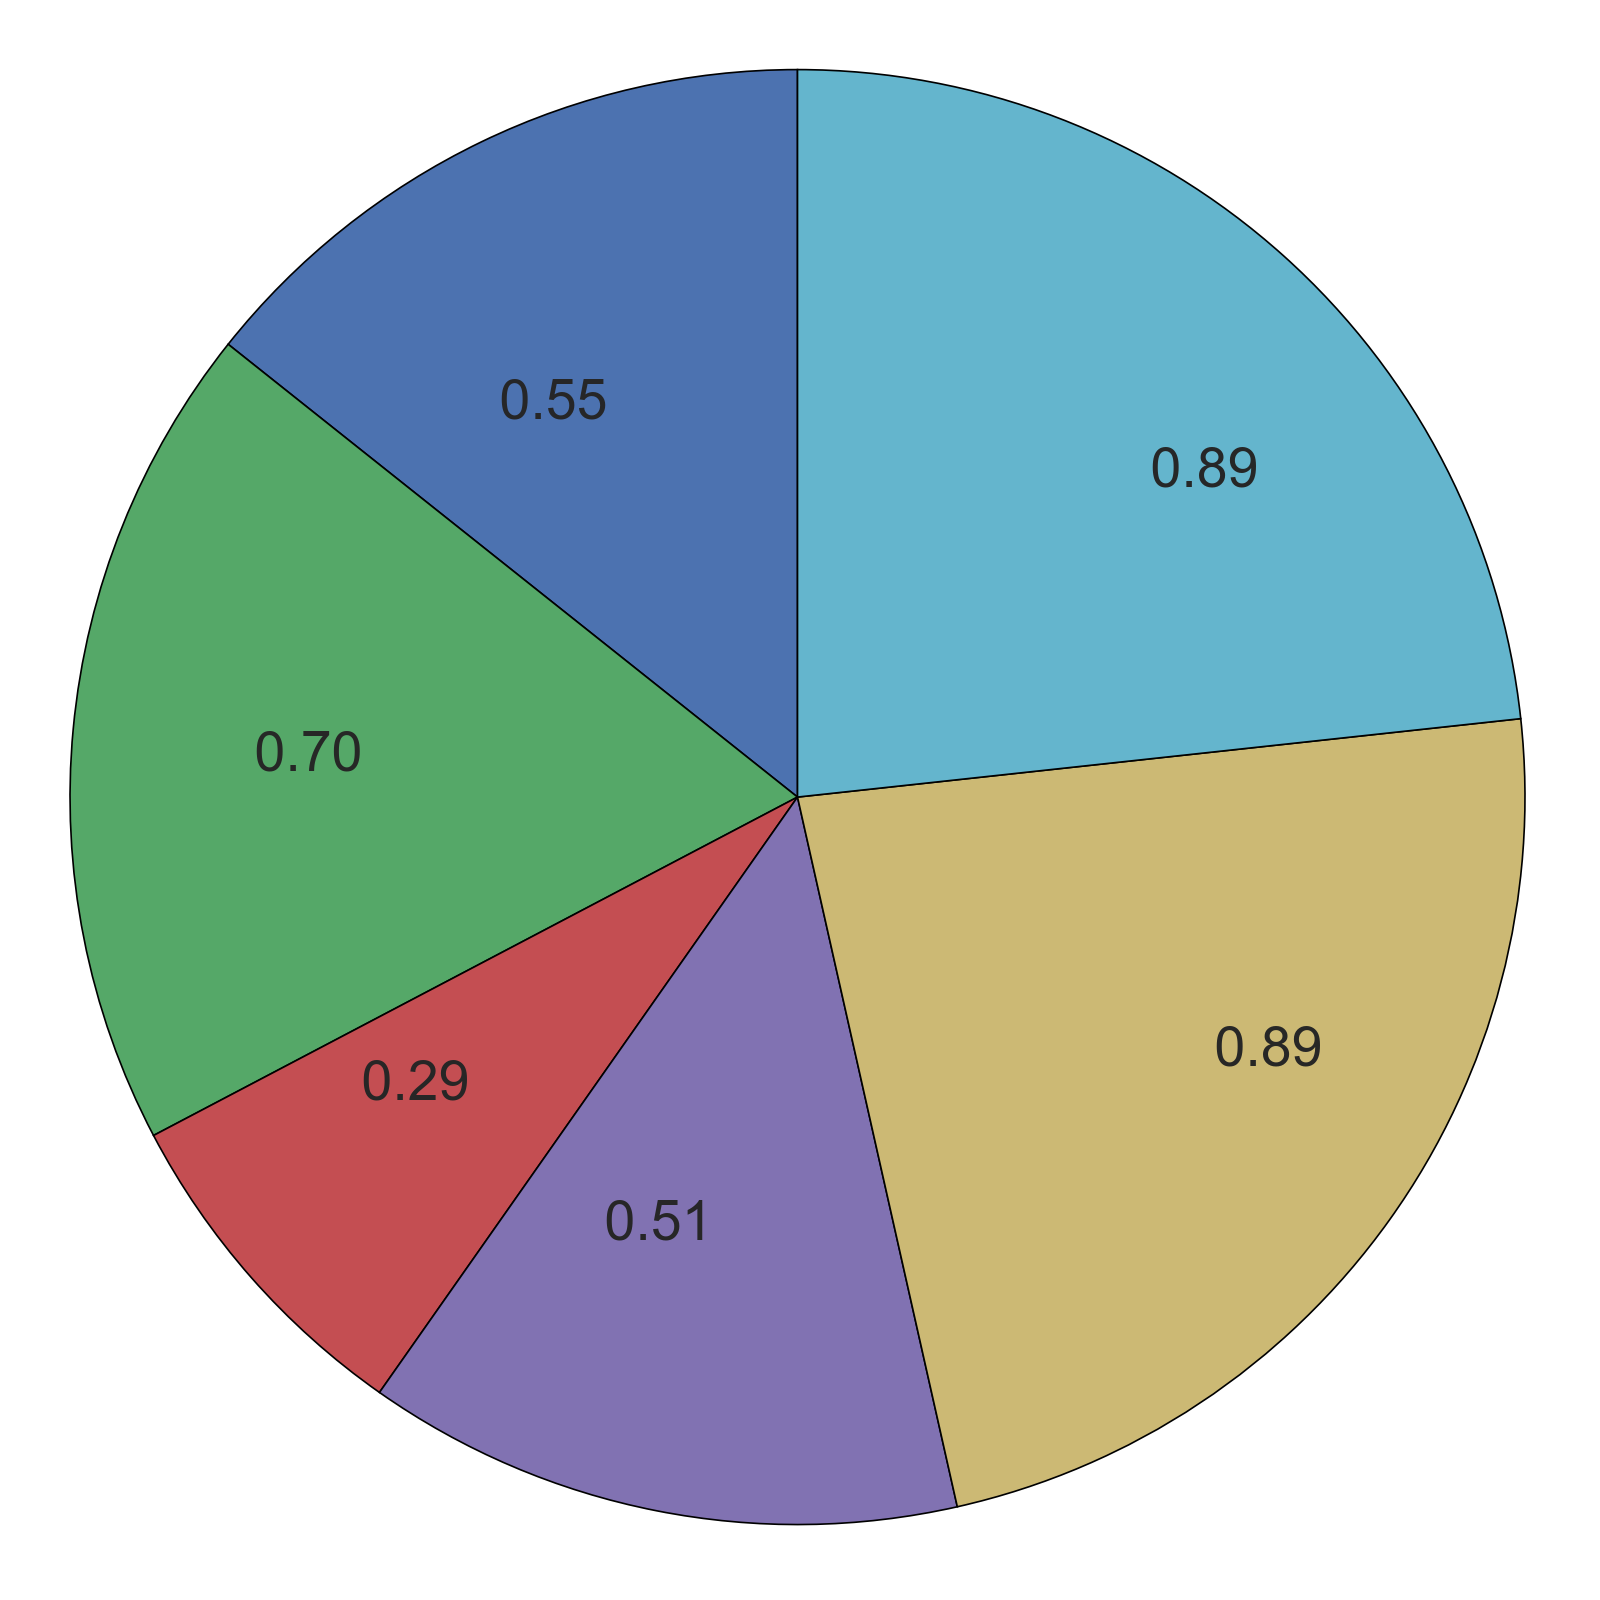
\includegraphics[width=\linewidth]{images/pie1.PNG}
				\onslide<6>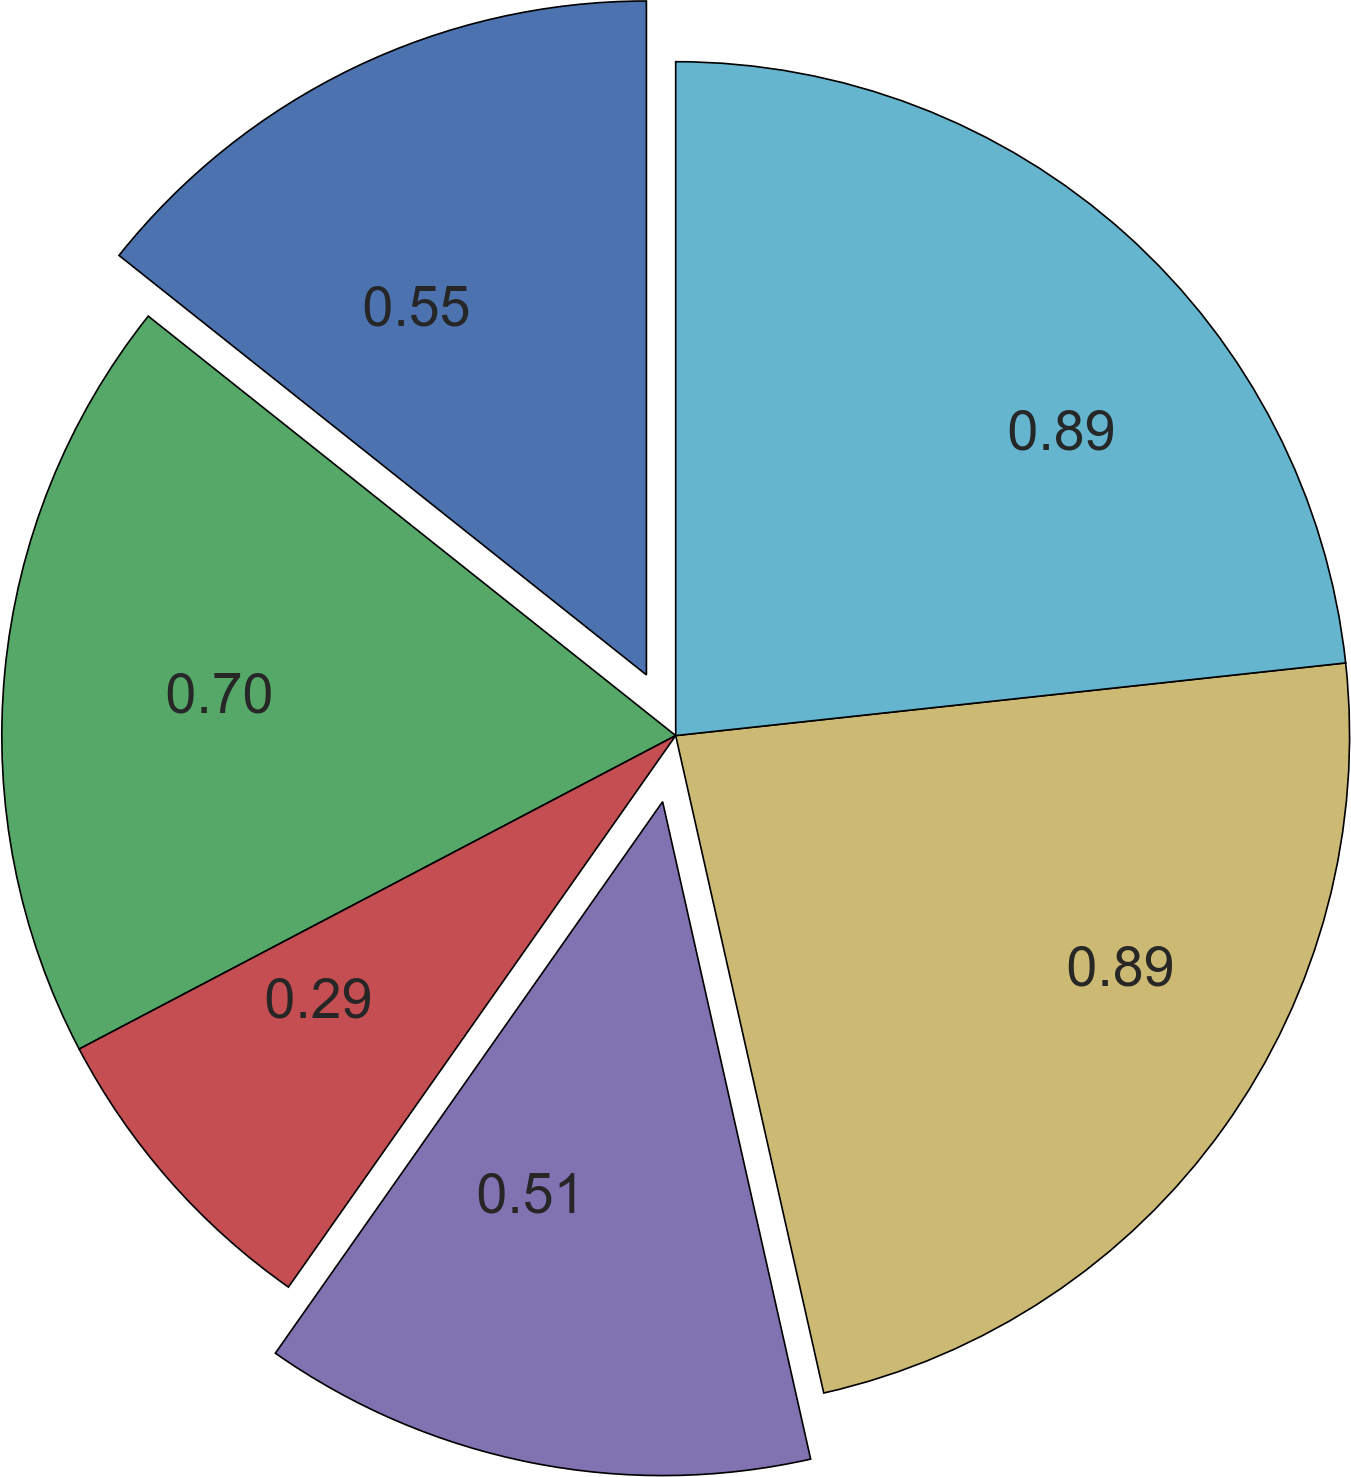
\includegraphics[width=\linewidth]{images/pie2.png}
			\end{overprint}
		\end{column}	
	\end{columns}
\end{frame}

{%
\setbeamertemplate{frame footer}{http://www.turingfinance.com/computational-finance
	
-updates-ieee-world-congress-computational-intelligence}
\begin{frame}{The Next Generation}
	\begin{itemize}[<+->]
		\item[]{
		\begin{figure}
			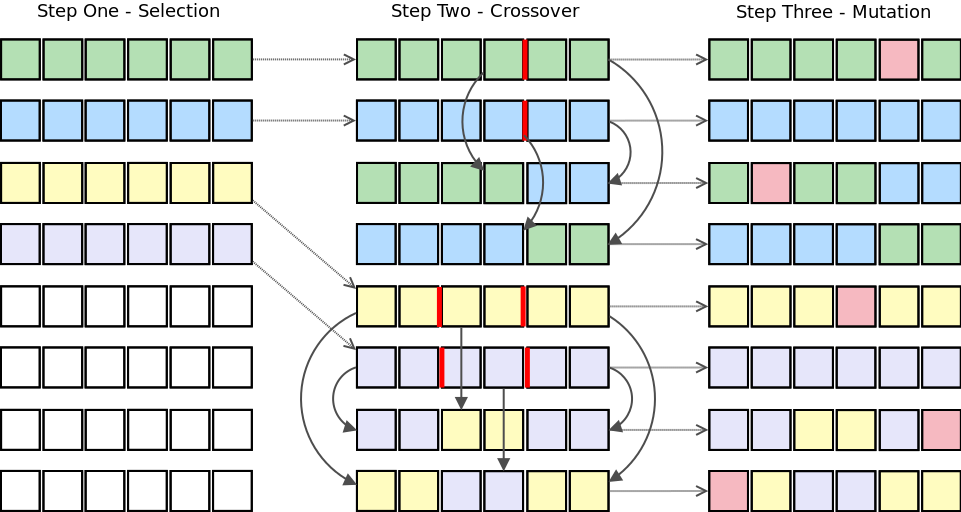
\includegraphics[width=0.9\linewidth]{images/Genes_turingFinance.png}
		\end{figure}}
		\item[]{~\\Crossover distinguishes this from Monte Carlo}
	\end{itemize}
\end{frame}
}


\begin{frame}{The Whole Algorithm}
	\begin{columns}[c] % align columns
		\begin{column}{.48\textwidth}
			\begin{itemize}[<+->]
				\item[1.] {Generate N random, sensible geometries}
				\item[2.] {Add each to blacklist}
				\item[3.] {Optimize each geometry}
				\item[4.] {Select Parents}
				\item[5.] {Crossover \& Mutate into sensible geometry}
				\item[6.] {Add Children to population}
				\item[7.] {Remove High energy individuals}
				\item[8.] {If converged:}
				\begin{itemize}
					\item{Done!}
				\end{itemize}
				\item[] {Otherwise:}
				\begin{itemize}
					\item{Go to 2}
				\end{itemize}
			\end{itemize}
		\end{column}
		\hfill
		\begin{column}{0.48\textwidth}
			\onslide<11>\begin{itemize}
				\item[]{
					\begin{figure}
						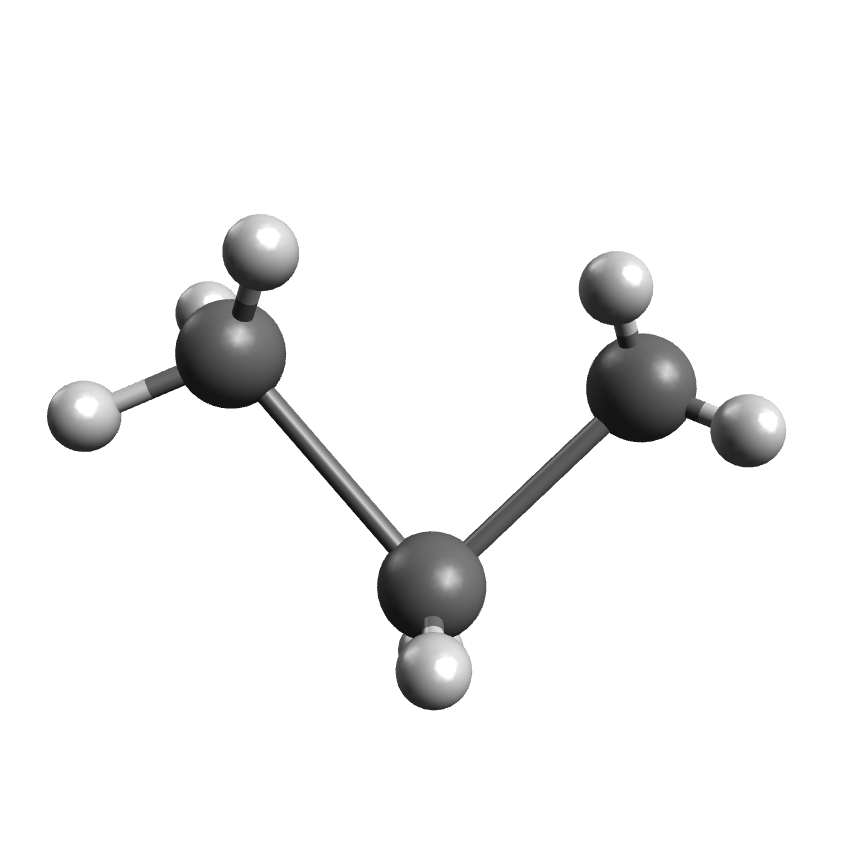
\includegraphics[width=0.7\linewidth]{images/sense.png}
						\caption*{sensible}
					\end{figure}
				}
			    \item[]{
			    	\begin{figure}
					    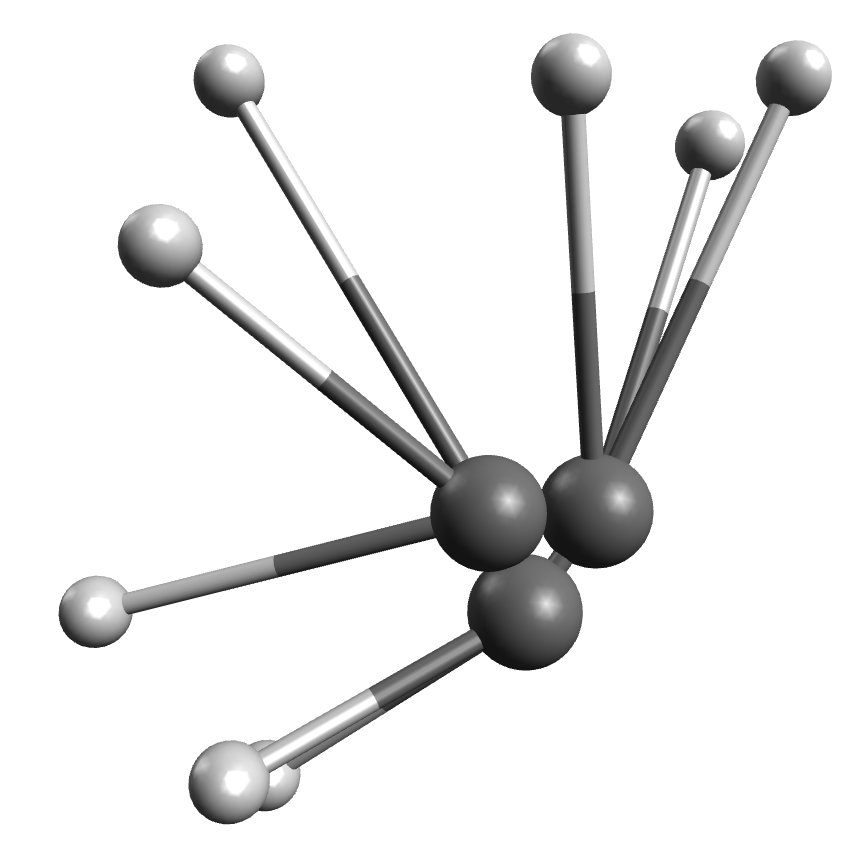
\includegraphics[width=0.7\linewidth]{images/nonsense.png}
					    \caption*{utter nonsense}
					\end{figure}
				}
			\end{itemize}
		\end{column}	
	\end{columns}
\end{frame}

\section{Finding Low Energy Conformers of Dipeptides}

{%
	\setbeamertemplate{frame footer}{Supady, A.; Blum, V.; Baldauf, C. J. Chem. Inf. Model. 2015, 55 (11), 2338–2348.}
\begin{frame}{Dipeptide Structures}
   	\begin{figure}
   		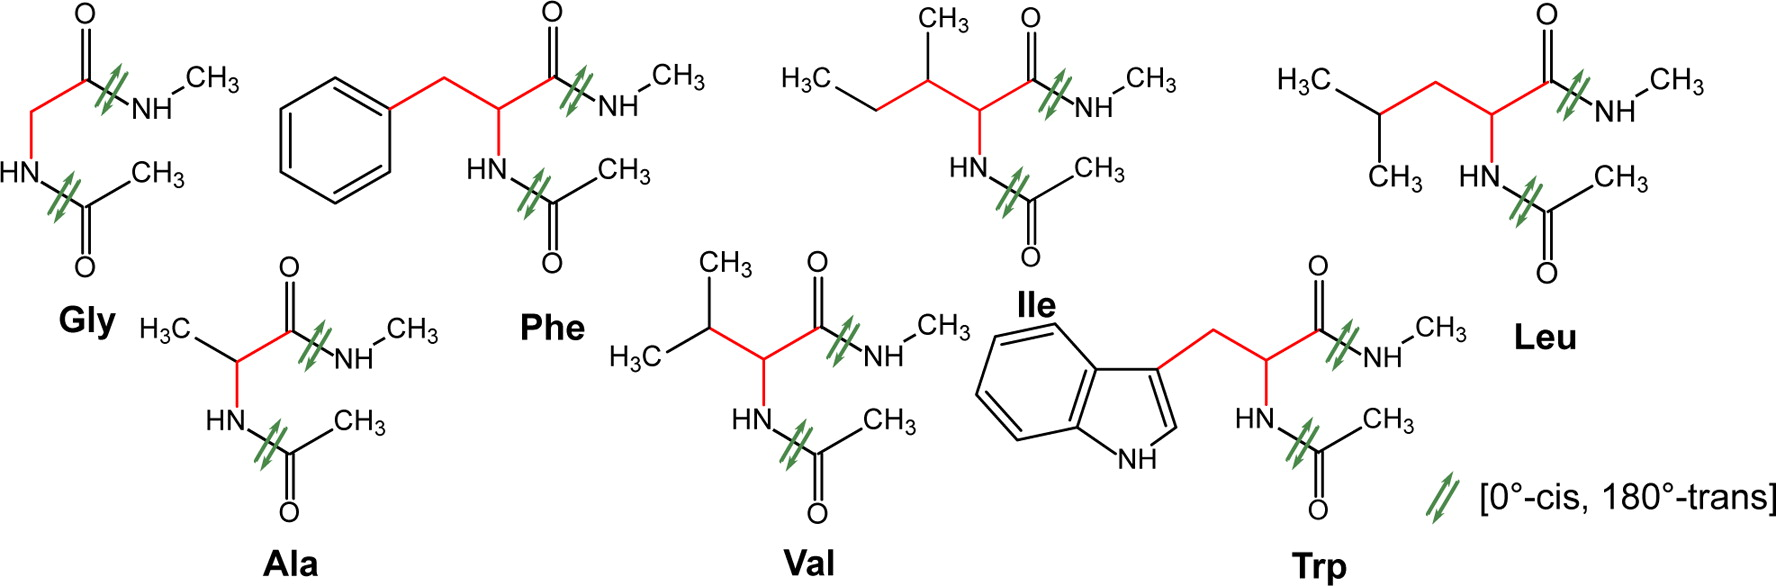
\includegraphics[width=\linewidth]{images/Supady2.jpeg}
   		\caption*{\textcolor{red}{Red} = Rotatable bonds \\
		   		  \textbf{\textcolor{darkgreen}{\ce{<=>}}} = Cis/Trans Bonds
		   		  }
   	\end{figure}
\end{frame}
}

{%
\setbeamertemplate{frame footer}{Supady, A.; Blum, V.; Baldauf, C. J. Chem. Inf. Model. 2015, 55 (11), 2338–2348.
}
\begin{frame}{Combinatorics}
	\begin{columns}[c] % align columns
		\begin{column}{.4\textwidth}
			\begin{itemize}
				\item {GA beats other methods if space is large}
				\item {Space gets large \textbf{\alert{fast}}}
			\end{itemize}		
		\end{column}
		\hfill
		\begin{column}{0.6\textwidth}
			\begin{figure}
				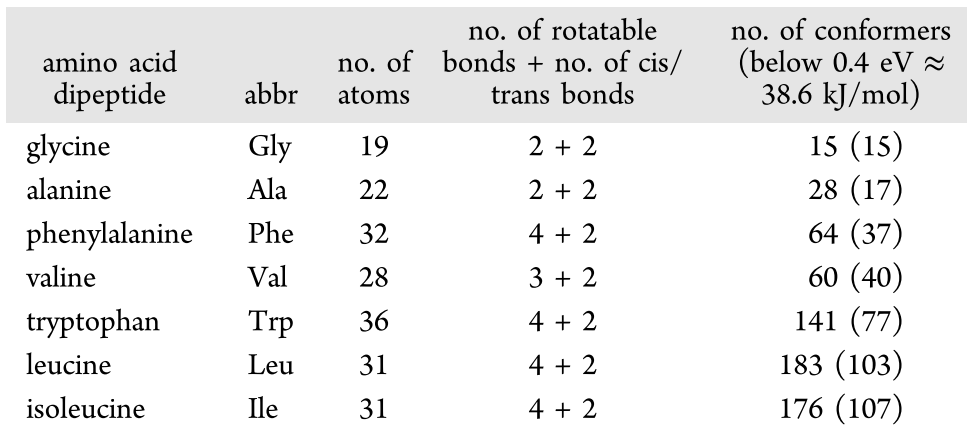
\includegraphics[width=\linewidth]{images/Confnums.png}
				% \caption*{\# of Conformers per dipeptide}
			\end{figure}
		\end{column}	
	\end{columns}
\end{frame}
}

{%
\setbeamertemplate{frame footer}{Supady, A.; Blum, V.; Baldauf, C. J. Chem. Inf. Model. 2015, 55 (11), 2338–2348.
}
\begin{frame}{Coverage}
	\begin{columns}[c] % align columns
		\begin{column}{.4\textwidth}
			\begin{itemize}
				\item {Smaller systems are reliably sampled}
				\item {As \# of conformers increases, miss more and more}
				\item {Is there a pattern to what is missed?}
			\end{itemize}		
		\end{column}
		\hfill
		\begin{column}{0.6\textwidth}
			\begin{figure}
				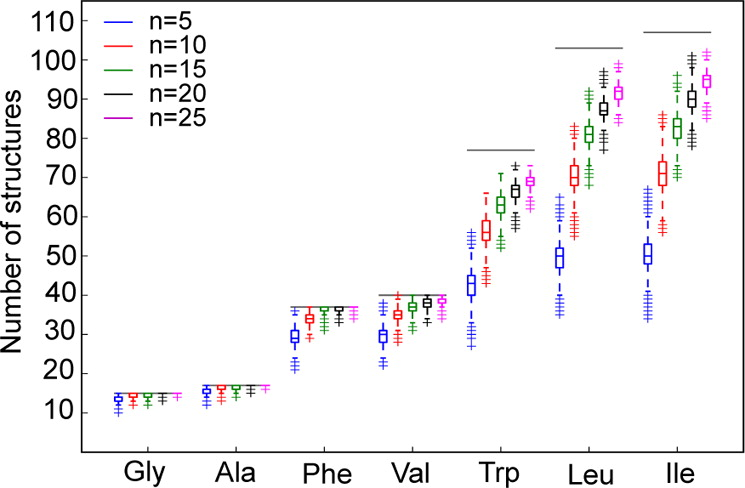
\includegraphics[width=\linewidth]{images/Supady4.jpeg}
				\caption*{Proportion of conformers found with incrasing runs of the GA}
			\end{figure}
		\end{column}	
	\end{columns}
\end{frame}
}

{%
\setbeamertemplate{frame footer}{Supady, A.; Blum, V.; Baldauf, C. J. Chem. Inf. Model. 2015, 55 (11), 2338–2348.
}
\begin{frame}{Coverage}
	\begin{columns}[c] % align columns
		\begin{column}{.4\textwidth}
			\begin{itemize}[<+->]
				\item {Most misses are very high energy}
				\item {Algorithm favors low energy areas of the space}
				\item {Features low in energy are favored and recombined}
			\end{itemize}		
		\end{column}
		\hfill
		\begin{column}{0.6\textwidth}
			\begin{figure}
				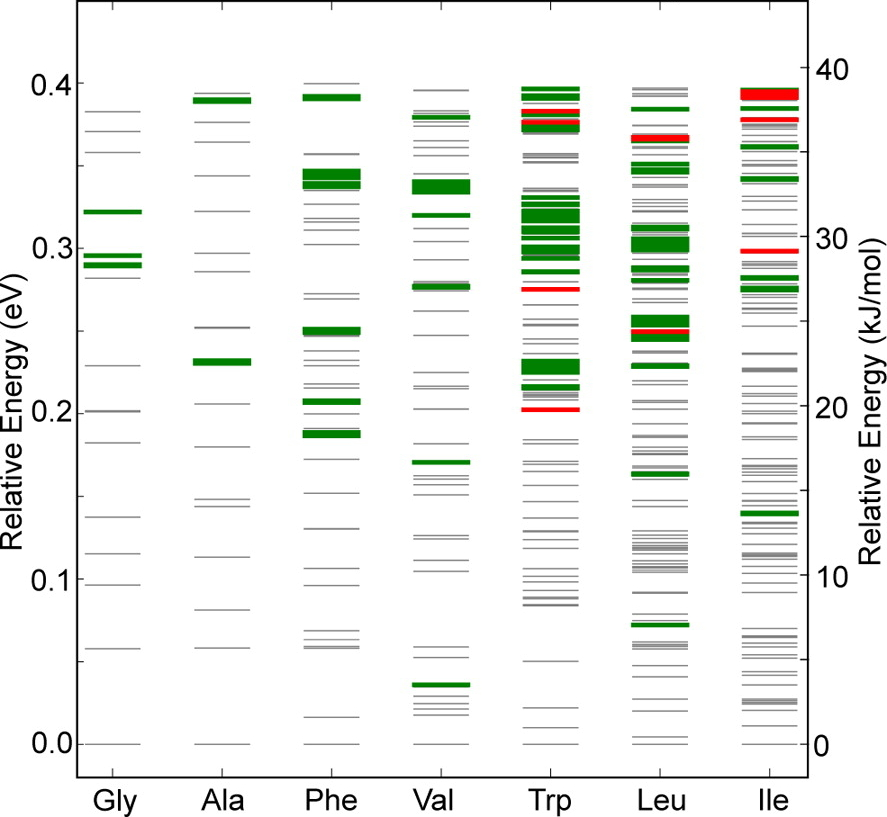
\includegraphics[width=0.75\linewidth]{images/Supady5.jpeg}
				\caption*{\textcolor{red}{---} Missed by the GA \\
				  \textcolor{darkgreen}{---} New Found by GA \\
				  \textcolor{gray}{---} In Reference \& GA}
			\end{figure}
		\end{column}	
	\end{columns}
\end{frame}
}

{%
\setbeamertemplate{frame footer}{Supady, A.; Blum, V.; Baldauf, C. J. Chem. Inf. Model. 2015, 55 (11), 2338–2348.}
\begin{frame}{Energy Cutoff}
	\begin{columns}[c] % align columns
		\begin{column}{.4\textwidth}
			\begin{itemize}[<+->]
				\item[] {
					\begin{figure}
					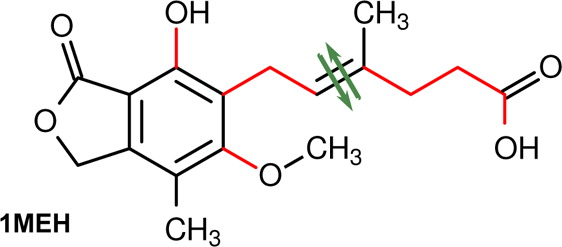
\includegraphics[width=\linewidth]{images/Supady3.jpeg}
					\caption*{Mycophenolic Acid}
					\end{figure}
				}
				\item {GA is more sensitive to energy cutoff}
				\item {For finding low energy ensemble, GA outperforms purely stochastic/deterministic method}
			\end{itemize}		
		\end{column}
		\hfill
		\begin{column}{0.6\textwidth}
			\begin{figure}
				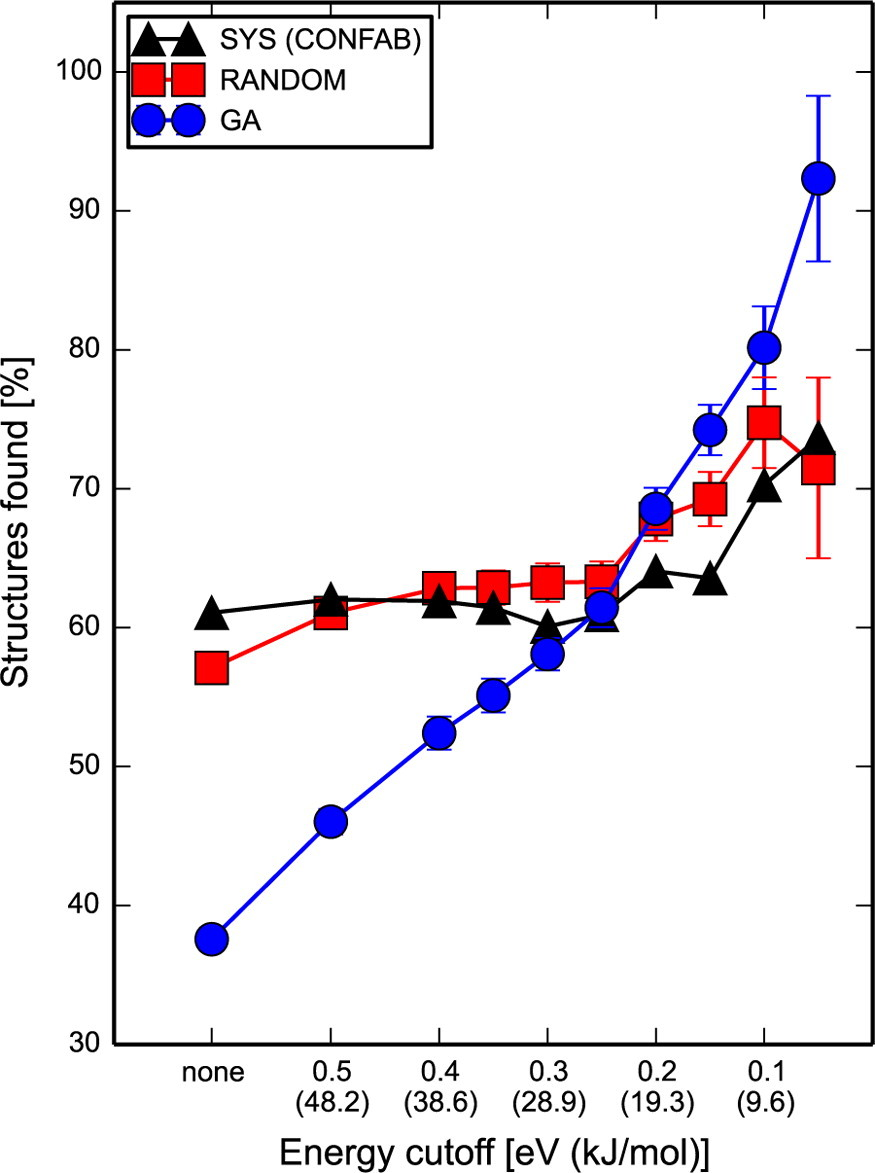
\includegraphics[width=0.75\linewidth]{images/Supady6.jpeg}
				%\caption*{\textcolor{red}{a}}
			\end{figure}
		\end{column}	
	\end{columns}
\end{frame}
}

\section{Concluding Remarks}

{%
\setbeamertemplate{frame footer}{Supady, A.; Blum, V.; Baldauf, C. J. Chem. Inf. Model. 2015, 55 (11), 2338–2348.}
\begin{frame}{Concluding Remarks}
	\begin{itemize}[<+->]
		\item {Finding all the low energy conformers for a molecule is hard}
		\item {In order to get accurate energies/structures, computationally expensive methods should be employed}
		\item {These take time, so we want to minimize how many of these we do}
		\item {The Genetic Algorithm provides a framework for a refined global search}
		\item {It shines when asked to find a host of low energy solutions}
		\item {GA wrapper can be interfaced with a variety of electronic structure packages(NWChem, ORCA) and is available under the GNU Lesser General Public License at \url{https://github.com/adrianasupady/fafoom}}
		
	\end{itemize}
\end{frame}
}


\begin{frame}[standout]
  Questions?
\end{frame}

\appendix

\begin{frame}[fragile]{Backup slide}
	\begin{itemize}
		\item Geometry optimization step makes the algorithm more Lamarckian (Jean Baptiste Larmarck, [1744-1829])
	\end{itemize}
\end{frame}

{%
\setbeamertemplate{frame footer}{(1) Blum, V. et. al., M. Comput. Phys. Commun. 2009, 180 (11), 2175–2196.
	
(2) Supady, A.; Blum, V.; Baldauf, C. J. Chem. Inf. Model. 2015, 55 (11), 2338–2348.

	}
\begin{frame}[fragile]{Genetic Algorithm Parameters}
	Geometry Optimization: DFT PBE + VdW, \emph{tier1} basis in FHI-aims$^1$.
	Convergence at 0.005 eV / \AA
	\begin{figure}
		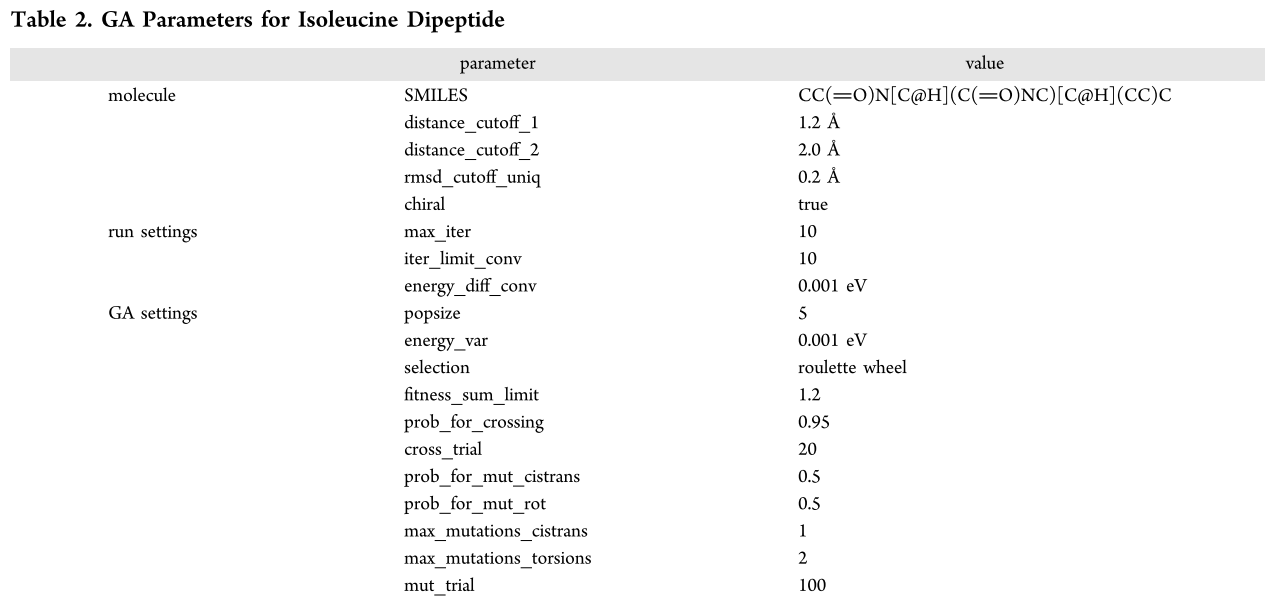
\includegraphics[width=\linewidth, trim={0 0 0 1.2cm},clip]{images/Params.png}
		\caption*{GA Parameters for Isoleucine Dipeptide$^2$}
	\end{figure}
\end{frame}
}
\end{document}
